\subsection{Past Paper 2023} 
\textbf{Data Structures, Algorithms \& Databases} \\
Answer ALL questions. Each question will be marked out of 20. The paper will be marked out of 80, which will be rescaled to a mark out of 100. [cite: 1]

\textbf{Question 1 Analysis of Algorithms and Tree Data Structures} \\
\textbf{Part 1} Consider a function named arrayToBST that takes an array of integers \textit{a} and inserts the elements of \textit{a} in an AVL tree \textit{T}. Therefore, function insert has re-balancing.
\begin{lstlisting}
Tree arrayToBST (int [] a) {
Tree T;
for (int i=0 i<a.length; i++) {
T = insert (T, a[i]);
}
return T;
}
\end{lstlisting} 

Is it possible to construct an input array \textit{a} of any arbitrary length \textit{n} that results in the outcomes described below? [cite: 3]
When it is possible to construct an input, give an example with length $n=8.$ [cite: 4]
\begin{enumerate}
    \item[(a)] Algorithm arrayToBST runs in time $\mathcal{O}(n).$ [cite: 4]
    \item[(b)] Algorithm arrayToBST runs in time $\mathcal{O}(n~log~n)$. [cite: 4]
    \item[(c)] Algorithm arrayToBST returns a perfectly balanced tree. [cite: 5]
\end{enumerate}
Briefly explain your construction. [cite: 5]
Note that your construction should apply to arrays with any arbitrary length \textit{n}; you cannot choose the length. [cite: 6] Your input array may or may not have repetitions. [cite: 7]

\textbf{Part 2} Consider a tree data structure where every node has at most three children: left child \textit{l}, middle child \textit{m} and right child \textit{r}. [cite: 8]
We call it a ternary tree. [cite: 9]
\begin{center}
\textit{X}
\\
\textit{l} \quad \textit{m} \quad \textit{r}
\end{center}
\begin{enumerate}
    \item[(d)] Give the maximum possible number of nodes of a ternary tree of height 4? [cite: 9, 10]
    \item[(e)] Give the minimum possible number of nodes of a ternary tree of height 4? [cite: 10, 11]
\end{enumerate}
Briefly explain how you compute these numbers. In particular, be clear about the definition of height you are using. [cite: 11]

\textbf{Question 2 Entity-Relationship modelling}

A company operates an online store where customers can place orders for various products, and has the following description of their requirements for a database: Customers need to provide details such as their name, email address, and shipping address to create an online account. [cite: 13] Each customer may have multiple orders, and each order is associated with only one customer. [cite: 14] An order contains one or more order items, where each order item represents a single product ordered by the customer. [cite: 15] An order item includes the quantity of the product ordered and its price at the time of purchase. [cite: 16] Each product has a unique product ID, a name, and a description. [cite: 17] Additionally, the company may track reviews for each product. A review includes the name of the reviewer, a rating, and a comment. [cite: 18] Each review is associated with only one product, and each product may have multiple reviews. [cite: 19] Finally, each order is associated with a payment. Each payment has a payment ID, an amount, a date and a payment method. [cite: 20]
\begin{enumerate}
    \item[(a)] Develop an Entity-Relationship model for the application. Explain the key design decisions made in your choice of entities, relationships and any other (ownership or hierarchical) aspects. [cite: 21] Annotate it with multiplicities and hierarchy annotations, as required. [cite: 22]
    \item[(b)] Carry out logical design for the model, representing the design with relational schemas for tables. [cite: 23, 24]
    \item[(c)] Write SQL CREATE TABLE statements for 2-3 tables. [cite: 24] Include among them a table that represents a relationship or incorporates a relationship, a weak entity or a subclass entity. [cite: 25] The other tables can be for the adjoining entities. [cite: 26]
\end{enumerate}

\textbf{Question 3 Graphs and Max-Heap Trees}

\textbf{Part 1} Consider the following weighted directed graph (with 7 vertices and 16 edges): [cite: 27]

\begin{figure}[h!]
    \centering
    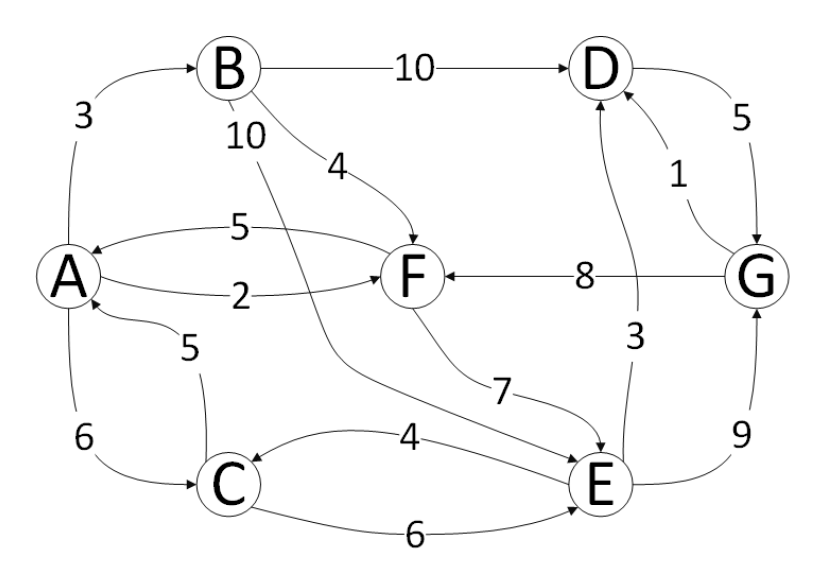
\includegraphics[width=0.8\textwidth]{unit-11/figures/dijkstra.png}
\end{figure}

\begin{enumerate}
    \item[(a)] Calculate the shortest path from A to G using the Dijkstra's algorithm. ("Shortest" means the path with the lowest total weight.) [cite: 28]
\end{enumerate}
You are expected to show your work using a table of the following form and also list the shortest path (e.g. A-\textgreater B-\textgreater) and and specify the resulting weight: [cite: 28]

\textbf{The following table:} 
\begin{tabular}{|c|c|c|c|c|c|c|c|}
\hline
A & B & C & D & E & F & G & Finished \\
\hline
0,A & $\infty$,B & $\infty$,C & $\infty$,D & $\infty$,E & $\infty$,F & $\infty$,G & \\
\hline
\end{tabular}

Total Weight: [cite: 30]
Shortest Path: [cite: 30]

\textbf{Part 2} Consider the complete binary tree below. Answer the following questions. [cite: 31]

% \begin{figure}[h!]
%     \centering
%     \includegraphics[width=0.8\textwidth]{image_31.png}
% \end{figure}

\textbf{(b)} In the process of building a Max-Heap Tree, the first swap is between \_\_\_ and \_\_\_ [2 marks] \\
 (write down the two numbers). \\
\textbf{(c)} And the second swap is between \_\_\_ and \_\_\_ [2 marks] \\
 (write down the two numbers). \\
\textbf{(d)} Draw the finished Max-Heap Tree (intermediate work is not required). [6 marks] \\

\textbf{Question 4 Relational algebra and normalisation} [cite: 34]

Consider the following schema for product sales for an online shop. [cite: 34]
\begin{verbatim}
product (pid, cat, price)
customer(cid, cname)
sale(pid, cid, date, qty)
\end{verbatim} [cite: 35]

("cat" is short for category and "qty" for quantity). [cite: 35] For estimating efficiency, assume around 100 products, 10,000 customers and several million sale records. [cite: 36]
\begin{enumerate}
    \item[(a)] State in English what the following relational algebra expression computes: [cite: 37]
    $$\pi_{cname}(\sigma_{qty*price\ge100}(\sigma_{cat=^{\prime}clothes^{\prime}}((product\gg customer)\gg sale)))$$
    \item[(b)] The expression given above is considered inefficient. [cite: 37] State all the ways in which it is inefficient. [cite: 38]
    \item[(c)] Give a more efficient version of the expression. [cite: 39] Make it as efficient as you can, and explain how it achieves efficiency. [cite: 39]
    \item[(d)] Consider a schema $T(A,B,C,D)$ with the functional dependencies $AB\longrightarrow C$ $AB\longrightarrow D$ and $BC\longrightarrow D$ [cite: 40]

    If we decompose the schema into (A, B, D) \& (B, C, D), is it a lossless decomposition? [cite: 40] If yes, explain why. If not, try to produce a counterexample. [cite: 41]

    Are the two subschemas in Boyce-Codd normal form? Explain. [cite: 41]
\end{enumerate}


\subsection{Past Paper 2024}
Answer ALL questions. Each question will be marked out of 20. The paper will be marked out of 80, which will be rescaled to a mark out of 100.

\textbf{Question 1 BST and AVL}

Let \_array = [20, 35, 5, 10, 18, 14, 35, 60, 75]. Consider a function named arrayToBST that takes \_array as the input and inserts the elements of array in a BST tree (without rebalancing)[cite: 2].
\begin{verbatim}
function arrayToBST(_array)

tree;

for element in array

tree insert (element, tree);

return tree;
\end{verbatim}
\begin{longtable}{|p{0.05\textwidth}|p{0.7\textwidth}|p{0.15\textwidth}|}
\hline
(a) & Draw the resulting tree. & [2 marks] \\
\hline
(b) & What is the height of the tree? & [2 marks] \\
\hline
(c) & Is it an AVL tree? Justify your answer. & [2 marks] \\
\hline
\end{longtable}

\begin{enumerate}
    \item[(d)] Consider a function named arrayToAVL that inserts the elements of array in an AVL tree[cite: 5]. The insert\_withRebalance() function will perform a rebalance if required[cite: 6].
\begin{verbatim}
function arrayToAVL(_array)

tree;

for element in array

tree insert_withRebalance (element, tree);

return tree;
\end{verbatim}
Use this function on array [20, 35, 5, 10, 18, 14, 35, 60, 75], show the results[cite: 7]. Illustrate the intermediate stages (before and after each rebalance) as well as the final tree[cite: 8]. [8 marks]
\end{enumerate}

\textbf{No calculator}

\begin{enumerate}
    \item[(e)] Here is a purported rebalance function that takes a node as the input[cite: 9]. Assume that \_node.left is the left subtree of a node; \_node.right is the right subtree of a node[cite: 10]; rightRotation() is a function that performs a left-to-right single rotation at a given node and leftRotation() similarly does a right-to-left single rotation[cite: 11].
\begin{verbatim}
function rebalance(_node)

if node has LL case imbalance

return leftRotation(_node.right)

if node has RR case imbalance
 return rightRotation(_node.left)

if node has LR case imbalance
 _node.right rightRotation(_node.left)
 return leftRotation(_node)

if node has RL case imbalance
 _node.left = leftRotation(_node.right)
 return rightRotation(_node)

return_node
\end{verbatim}
There are errors/bugs in the above pseudo-code which lead to a wrong rebalance result[cite: 12]. Write the corrected pseudo-code in the same style[cite: 13]. [6 marks]
\end{enumerate}

\textbf{No calculator}

\textbf{Question 2 Entity-Relationship modelling}

A database is required for an airline flight reservation system[cite: 14]. This system enables customers to book flights by selecting the flight number, origin, destination, departure date, and time[cite: 15]. Each booking is assigned a unique booking ID number and contains booking for multiple passengers[cite: 16]. The airline allocates baggage allowance for the booking, in terms of the number of pieces of baggage which may depend on the frequent flyer status of the customer[cite: 17].
\begin{enumerate}
    \item[(a)] Develop an Entity-Relationship model for the application[cite: 18]. Explain the key design decisions made in your choice of entities, relationships and any other (ownership or hierarchical) aspects[cite: 18]. Annotate it with multiplicities and hierarchy annotations, as required[cite: 19]. [10 marks]
    \item[(b)] Carry out logical design for the model, representing the design with relational schemas for tables[cite: 20]. Annotate the schemas with primary keys and the possibility of null attributes[cite: 20]. [5 marks]
    \item[(c)] Write CREATE TABLE statements for 2-3 tables[cite: 21]. Include among them a table that represents a relationship or incorporates a relationship, a weak entity or a subclass entity[cite: 21]. The other table(s) may be those that are linked to this table[cite: 22]. [5 marks]
\end{enumerate}

\textbf{No calculator}

\textbf{Question 3 Graphs and Max-Heap Trees}

\begin{enumerate}
    \item[(a)] Consider the following weighted directed graph:
    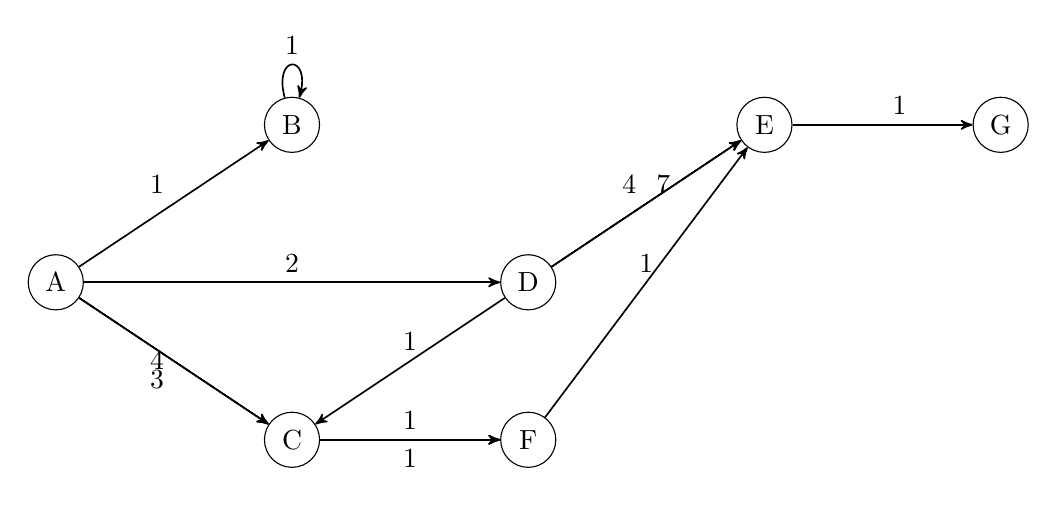
\begin{tikzpicture}
        \usetikzlibrary{arrows, positioning}
        \tikzset{
            vertex/.style={circle, draw, minimum size=0.7cm},
            edge/.style={->, >=stealth', semithick}
        }

        % Nodes
        \node[vertex] (A) at (0,0) {A};
        \node[vertex] (B) at (3,2) {B};
        \node[vertex] (D) at (6,0) {D};
        \node[vertex] (C) at (3,-2) {C};
        \node[vertex] (E) at (9,2) {E};
        \node[vertex] (F) at (6,-2) {F};
        \node[vertex] (G) at (12,2) {G};

        % Edges
        \draw[edge] (A) to node[above left] {1} (B);
        \draw[edge] (A) to node[above] {2} (D);
        \draw[edge] (A) to node[below left] {3} (C);
        \draw[edge] (A) to node[left] {4} (C); % Duplicate edge for better visualization if needed, otherwise combine weights.
        \draw[edge] (B) to [loop above] node {1} (B);
        \draw[edge] (D) to node[above left] {4} (E);
        \draw[edge] (D) to node[above right] {7} (E); % Duplicate edge for better visualization if needed, otherwise combine weights.
        \draw[edge] (D) to node[above] {1} (C);
        \draw[edge] (C) to node[above] {1} (F);
        \draw[edge] (C) to node[below] {1} (F); % Duplicate edge for better visualization if needed, otherwise combine weights.
        \draw[edge] (E) to node[above right] {1} (G);
        \draw[edge] (F) to node[above] {1} (E);
    \end{tikzpicture}

    Calculate the shortest path from A to G using the Dijkstra's algorithm[cite: 24]. ("Shortest" means the path with the lowest total weight.) [cite: 24] [10 marks]

    You are expected to show your work using a table of the following form and also list the shortest path (e.g. A$\rightarrow$B$\rightarrow$C) and and specify the resulting weight:

    \textbf{The following table:}
    \begin{longtable}{|c|c|c|c|c|c|c|c|}
    \hline
    A & B & C & D & E & F & G & Finished \\
    \hline
    0,A & $\infty$,B & $\infty$,C & $\infty$,D & $\infty$,E & $\infty$,F & $\infty$,G & \\
    \hline
    & & & & & & & \\
    \hline
    & & & & & & & \\
    \hline
    & & & & & & & \\
    \hline
    & & & & & & & \\
    \hline
    & & & & & & & \\
    \hline
    & & & & & & & \\
    \hline
    \end{longtable}

    Total Weight:
    Shortest Path:
\end{enumerate}

\textbf{No calculator}

Consider the following algorithm and let n be the length of array[cite: 25].
\begin{verbatim}
def insert_all(array):

d = <empty data structure>

for x in array:

<insert x in data structure d>
\end{verbatim}
\begin{enumerate}
    \item[(b)] Suppose d is a binary search tree, without balancing[cite: 27]. Give the time complexity of insert all as a function of n in "big-Oh" or $O()$ notation[cite: 27]. [3 marks]
    \item[(c)] Suppose d is a hash table[cite: 29]. Give the time complexity of insert all as a function of n in "big-Oh" or $O()$ notation[cite: 29]. [3 marks]
    \item[(d)] Does there exist an input array for which insert all has same time complexity, regardless of whether d is a binary search tree or d is a hash table? [cite: 30] If the answer is yes, give an example array of length $n=7$[cite: 30]. If the answer if no, motivate your answer[cite: 30]. [4 marks]
\end{enumerate}

\textbf{Question 4 Relational algebra and normalisation}

Consider the following schemas for a database used by a student registration system.

\textbf{The following table:}
\begin{longtable}{|l|l|}
\hline
\textbf{Table} & \textbf{course} \\
\hline
cid & integer \\
\hline
title & varchar(40) \\
\hline
level & integer \\
\hline
\end{longtable}

\textbf{Table prerequisite}
\begin{verbatim}
pre Integer
post integer
\end{verbatim}

\textbf{The following table:}
\begin{longtable}{|l|l|l|l|}
\hline
\textbf{Table} & \textbf{student} & & \textbf{Table registered} \\
\hline
sid & integer & sid & integer \\
\hline
name & varchar(40) & cid & integer \\
\hline
& & year & integer \\
\hline
\end{longtable}

The table prerequisite describes prerequisites for courses, indicating that a "pre" course must be taken before taking a "post" course (Both "pre" and "post" are course ids)[cite: 36]. For example a course called "Programming 1" might be a prerequisite for a course called "Programming 2"[cite: 37]. In general, a course may have any number of prerequisites[cite: 38]. The table registered describes which students have registered for which courses in a particular year[cite: 39].
\begin{enumerate}
    \item[(a)] Write a relational algebra expression for the following problem:

    Find the ID numbers of students who took some level 2 course in 2023. [2 marks]

    \item[(b)] Write a relational algebra expression for the following problem:

    Find the ID numbers of students who took only level 2 courses in 2023. Or, to put another way, find the ID numbers of students who registered for courses all of which are at level 2. [4 marks]

    Hint: You may find the following logical equivalence useful in devising your solution:

    for all x, P $\rightarrow$ not (exists x such that not P)

    \item[(c)] Explain in words what the following expression calculates[cite: 41]:
    $$\pi_{pre,post}(\rho_{(pre;cid)}(prerequisite)\gg\rho_{(cid,post)}(prerequisite))$$
    [4 marks]

    \item[(d)] Define precisely when a set of tables is said to be in Boyce-Codd normal form[cite: 42]. [4 marks]
    \item[(e)] Consider an employee table with the schema:

    employee(last\_name, first\_name, office, phone\_number)
    and the functional dependency phone\_number $\rightarrow$ office[cite: 43]. Explain the possibility of update anomaly and deletion anomaly arising from this dependency, giving examples of situations that would lead to the anomalies[cite: 44]. [4 marks]

    How does the use of Boyce-Codd normal form avoid these anomalies? [2 marks]
\end{enumerate}
